\documentclass[1p]{elsarticle_modified}
%\bibliographystyle{elsarticle-num}

%\usepackage[colorlinks]{hyperref}
%\usepackage{abbrmath_seonhwa} %\Abb, \Ascr, \Acal ,\Abf, \Afrak
\usepackage{amsfonts}
\usepackage{amssymb}
\usepackage{amsmath}
\usepackage{amsthm}
\usepackage{scalefnt}
\usepackage{amsbsy}
\usepackage{kotex}
\usepackage{caption}
\usepackage{subfig}
\usepackage{color}
\usepackage{graphicx}
\usepackage{xcolor} %% white, black, red, green, blue, cyan, magenta, yellow
\usepackage{float}
\usepackage{setspace}
\usepackage{hyperref}

\usepackage{tikz}
\usetikzlibrary{arrows}

\usepackage{multirow}
\usepackage{array} % fixed length table
\usepackage{hhline}

%%%%%%%%%%%%%%%%%%%%%
\makeatletter
\renewcommand*\env@matrix[1][\arraystretch]{%
	\edef\arraystretch{#1}%
	\hskip -\arraycolsep
	\let\@ifnextchar\new@ifnextchar
	\array{*\c@MaxMatrixCols c}}
\makeatother %https://tex.stackexchange.com/questions/14071/how-can-i-increase-the-line-spacing-in-a-matrix
%%%%%%%%%%%%%%%

\usepackage[normalem]{ulem}

\newcommand{\msout}[1]{\ifmmode\text{\sout{\ensuremath{#1}}}\else\sout{#1}\fi}
%SOURCE: \msout is \stkout macro in https://tex.stackexchange.com/questions/20609/strikeout-in-math-mode

\newcommand{\cancel}[1]{
	\ifmmode
	{\color{red}\msout{#1}}
	\else
	{\color{red}\sout{#1}}
	\fi
}

\newcommand{\add}[1]{
	{\color{blue}\uwave{#1}}
}

\newcommand{\replace}[2]{
	\ifmmode
	{\color{red}\msout{#1}}{\color{blue}\uwave{#2}}
	\else
	{\color{red}\sout{#1}}{\color{blue}\uwave{#2}}
	\fi
}

\newcommand{\Sol}{\mathcal{S}} %segment
\newcommand{\D}{D} %diagram
\newcommand{\A}{\mathcal{A}} %arc


%%%%%%%%%%%%%%%%%%%%%%%%%%%%%5 test

\def\sl{\operatorname{\textup{SL}}(2,\Cbb)}
\def\psl{\operatorname{\textup{PSL}}(2,\Cbb)}
\def\quan{\mkern 1mu \triangleright \mkern 1mu}

\theoremstyle{definition}
\newtheorem{thm}{Theorem}[section]
\newtheorem{prop}[thm]{Proposition}
\newtheorem{lem}[thm]{Lemma}
\newtheorem{ques}[thm]{Question}
\newtheorem{cor}[thm]{Corollary}
\newtheorem{defn}[thm]{Definition}
\newtheorem{exam}[thm]{Example}
\newtheorem{rmk}[thm]{Remark}
\newtheorem{alg}[thm]{Algorithm}

\newcommand{\I}{\sqrt{-1}}
\begin{document}

%\begin{frontmatter}
%
%\title{Boundary parabolic representations of knots up to 8 crossings}
%
%%% Group authors per affiliation:
%\author{Yunhi Cho} 
%\address{Department of Mathematics, University of Seoul, Seoul, Korea}
%\ead{yhcho@uos.ac.kr}
%
%
%\author{Seonhwa Kim} %\fnref{s_kim}}
%\address{Center for Geometry and Physics, Institute for Basic Science, Pohang, 37673, Korea}
%\ead{ryeona17@ibs.re.kr}
%
%\author{Hyuk Kim}
%\address{Department of Mathematical Sciences, Seoul National University, Seoul 08826, Korea}
%\ead{hyukkim@snu.ac.kr}
%
%\author{Seokbeom Yoon}
%\address{Department of Mathematical Sciences, Seoul National University, Seoul, 08826,  Korea}
%\ead{sbyoon15@snu.ac.kr}
%
%\begin{abstract}
%We find all boundary parabolic representation of knots up to 8 crossings.
%
%\end{abstract}
%\begin{keyword}
%    \MSC[2010] 57M25 
%\end{keyword}
%
%\end{frontmatter}

%\linenumbers
%\tableofcontents
%
\newcommand\colored[1]{\textcolor{white}{\rule[-0.35ex]{0.8em}{1.4ex}}\kern-0.8em\color{red} #1}%
%\newcommand\colored[1]{\textcolor{white}{ #1}\kern-2.17ex	\textcolor{white}{ #1}\kern-1.81ex	\textcolor{white}{ #1}\kern-2.15ex\color{red}#1	}

{\Large $\underline{12n_{0810}~(K12n_{0810})}$}

\setlength{\tabcolsep}{10pt}
\renewcommand{\arraystretch}{1.6}
\vspace{1cm}\begin{tabular}{m{100pt}>{\centering\arraybackslash}m{274pt}}
\multirow{5}{120pt}{
	\centering
	\includegraphics[width=112pt]{../../../GIT/diagram.site/Diagrams/png/2899_12n_0810.png}\\
\ \ \ A knot diagram\footnotemark}&
\allowdisplaybreaks
\textbf{Linearized knot diagam} \\
\cline{2-2}
 &
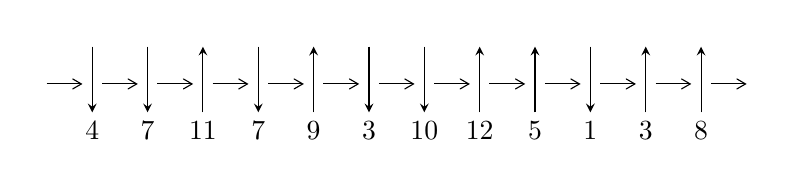
\begin{tikzpicture}[x=20pt, y=17pt]
	% nodes
	\node (C0) at (0, 0) {};
	\node (C1) at (1, 0) {};
	\node (C1U) at (1, +1) {};
	\node (C1D) at (1, -1) {4};

	\node (C2) at (2, 0) {};
	\node (C2U) at (2, +1) {};
	\node (C2D) at (2, -1) {7};

	\node (C3) at (3, 0) {};
	\node (C3U) at (3, +1) {};
	\node (C3D) at (3, -1) {11};

	\node (C4) at (4, 0) {};
	\node (C4U) at (4, +1) {};
	\node (C4D) at (4, -1) {7};

	\node (C5) at (5, 0) {};
	\node (C5U) at (5, +1) {};
	\node (C5D) at (5, -1) {9};

	\node (C6) at (6, 0) {};
	\node (C6U) at (6, +1) {};
	\node (C6D) at (6, -1) {3};

	\node (C7) at (7, 0) {};
	\node (C7U) at (7, +1) {};
	\node (C7D) at (7, -1) {10};

	\node (C8) at (8, 0) {};
	\node (C8U) at (8, +1) {};
	\node (C8D) at (8, -1) {12};

	\node (C9) at (9, 0) {};
	\node (C9U) at (9, +1) {};
	\node (C9D) at (9, -1) {5};

	\node (C10) at (10, 0) {};
	\node (C10U) at (10, +1) {};
	\node (C10D) at (10, -1) {1};

	\node (C11) at (11, 0) {};
	\node (C11U) at (11, +1) {};
	\node (C11D) at (11, -1) {3};

	\node (C12) at (12, 0) {};
	\node (C12U) at (12, +1) {};
	\node (C12D) at (12, -1) {8};
	\node (C13) at (13, 0) {};

	% arrows
	\draw[->,>={angle 60}]
	(C0) edge (C1) (C1) edge (C2) (C2) edge (C3) (C3) edge (C4) (C4) edge (C5) (C5) edge (C6) (C6) edge (C7) (C7) edge (C8) (C8) edge (C9) (C9) edge (C10) (C10) edge (C11) (C11) edge (C12) (C12) edge (C13) ;	\draw[->,>=stealth]
	(C1U) edge (C1D) (C2U) edge (C2D) (C3D) edge (C3U) (C4U) edge (C4D) (C5D) edge (C5U) (C6U) edge (C6D) (C7U) edge (C7D) (C8D) edge (C8U) (C9D) edge (C9U) (C10U) edge (C10D) (C11D) edge (C11U) (C12D) edge (C12U) ;
	\end{tikzpicture} \\
\hhline{~~} \\& 
\textbf{Solving Sequence} \\ \cline{2-2} 
 &
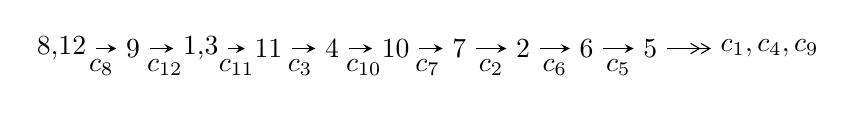
\begin{tikzpicture}[x=23pt, y=7pt]
	% node
	\node (A0) at (-1/8, 0) {8,12};
	\node (A1) at (1, 0) {9};
	\node (A2) at (33/16, 0) {1,3};
	\node (A3) at (25/8, 0) {11};
	\node (A4) at (33/8, 0) {4};
	\node (A5) at (41/8, 0) {10};
	\node (A6) at (49/8, 0) {7};
	\node (A7) at (57/8, 0) {2};
	\node (A8) at (65/8, 0) {6};
	\node (A9) at (73/8, 0) {5};
	\node (C1) at (1/2, -1) {$c_{8}$};
	\node (C2) at (3/2, -1) {$c_{12}$};
	\node (C3) at (21/8, -1) {$c_{11}$};
	\node (C4) at (29/8, -1) {$c_{3}$};
	\node (C5) at (37/8, -1) {$c_{10}$};
	\node (C6) at (45/8, -1) {$c_{7}$};
	\node (C7) at (53/8, -1) {$c_{2}$};
	\node (C8) at (61/8, -1) {$c_{6}$};
	\node (C9) at (69/8, -1) {$c_{5}$};
	\node (A10) at (11, 0) {$c_{1},c_{4},c_{9}$};

	% edge
	\draw[->,>=stealth]	
	(A0) edge (A1) (A1) edge (A2) (A2) edge (A3) (A3) edge (A4) (A4) edge (A5) (A5) edge (A6) (A6) edge (A7) (A7) edge (A8) (A8) edge (A9) ;
	\draw[->>,>={angle 60}]	
	(A9) edge (A10);
\end{tikzpicture} \\ 

\end{tabular} \\

\footnotetext{
The image of knot diagram is generated by the software ``\textbf{Draw programme}" developed by Andrew Bartholomew(\url{http://www.layer8.co.uk/maths/draw/index.htm\#Running-draw}), where we modified some parts for our purpose(\url{https://github.com/CATsTAILs/LinksPainter}).
}\phantom \\ \newline 
\centering \textbf{Ideals for irreducible components\footnotemark of $X_{\text{par}}$} 
 
\begin{align*}
I^u_{1}&=\langle 
46649848211422 u^{20}-271752392335713 u^{19}+\cdots+2892575498427142 b-407290304844750,\\
\phantom{I^u_{1}}&\phantom{= \langle  }616531903691785 u^{20}-4456755156074076 u^{19}+\cdots+5785150996854284 a-8643983373087020,\\
\phantom{I^u_{1}}&\phantom{= \langle  }u^{21}-8 u^{20}+\cdots+4 u-4\rangle \\
I^u_{2}&=\langle 
17 u^{13} a+3 u^{13}+\cdots+90 a-135,\;15 u^{13} a+26 u^{13}+\cdots+180 a+160,\\
\phantom{I^u_{2}}&\phantom{= \langle  }u^{14}-2 u^{13}+8 u^{12}-13 u^{11}+26 u^{10}-32 u^9+44 u^8-40 u^7+42 u^6-25 u^5+25 u^4-7 u^3+10 u^2+2\rangle \\
I^u_{3}&=\langle 
934420413114 u^{21} a-2562507066002 u^{21}+\cdots-20080961710080 a+99672371759230,\\
\phantom{I^u_{3}}&\phantom{= \langle  }-58418953866728 u^{21} a+52781909440645 u^{21}+\cdots+613677712103440 a-532451057055698,\\
\phantom{I^u_{3}}&\phantom{= \langle  }u^{22}+3 u^{21}+\cdots-106 u-16\rangle \\
I^u_{4}&=\langle 
-11 u^9-27 u^8-72 u^7-123 u^6-201 u^5-298 u^4-405 u^3-392 u^2+4 b-238 u-64,\\
\phantom{I^u_{4}}&\phantom{= \langle  }127 u^9+288 u^8+805 u^7+1315 u^6+2210 u^5+3201 u^4+4367 u^3+4163 u^2+52 a+2522 u+694,\\
\phantom{I^u_{4}}&\phantom{= \langle  }u^{10}+3 u^9+8 u^8+15 u^7+25 u^6+38 u^5+53 u^4+58 u^3+44 u^2+20 u+4\rangle \\
\\
\end{align*}
\raggedright * 4 irreducible components of $\dim_{\mathbb{C}}=0$, with total 103 representations.\\
\footnotetext{All coefficients of polynomials are rational numbers. But the coefficients are sometimes approximated in decimal forms when there is not enough margin.}
\newpage
\renewcommand{\arraystretch}{1}
\centering \section*{I. $I^u_{1}= \langle 4.66\times10^{13} u^{20}-2.72\times10^{14} u^{19}+\cdots+2.89\times10^{15} b-4.07\times10^{14},\;6.17\times10^{14} u^{20}-4.46\times10^{15} u^{19}+\cdots+5.79\times10^{15} a-8.64\times10^{15},\;u^{21}-8 u^{20}+\cdots+4 u-4 \rangle$}
\flushleft \textbf{(i) Arc colorings}\\
\begin{tabular}{m{7pt} m{180pt} m{7pt} m{180pt} }
\flushright $a_{8}=$&$\begin{pmatrix}1\\0\end{pmatrix}$ \\
\flushright $a_{12}=$&$\begin{pmatrix}0\\u\end{pmatrix}$ \\
\flushright $a_{9}=$&$\begin{pmatrix}1\\- u^2\end{pmatrix}$ \\
\flushright $a_{1}=$&$\begin{pmatrix}u\\u\end{pmatrix}$ \\
\flushright $a_{3}=$&$\begin{pmatrix}-0.106571 u^{20}+0.770378 u^{19}+\cdots-10.1014 u+1.49417\\-0.0161274 u^{20}+0.0939482 u^{19}+\cdots-1.66730 u+0.140805\end{pmatrix}$ \\
\flushright $a_{11}=$&$\begin{pmatrix}0.138515 u^{20}-1.16208 u^{19}+\cdots-0.849168 u-2.59979\\0.0651459 u^{20}-0.521592 u^{19}+\cdots+2.89327 u-0.507601\end{pmatrix}$ \\
\flushright $a_{4}=$&$\begin{pmatrix}-0.305406 u^{20}+2.43760 u^{19}+\cdots+3.23821 u-0.643820\\-0.115389 u^{20}+0.953768 u^{19}+\cdots+0.0723902 u+0.582350\end{pmatrix}$ \\
\flushright $a_{10}=$&$\begin{pmatrix}0.126900 u^{20}-1.08035 u^{19}+\cdots-1.35677 u-2.38567\\0.0535308 u^{20}-0.439861 u^{19}+\cdots+2.38567 u-0.293478\end{pmatrix}$ \\
\flushright $a_{7}=$&$\begin{pmatrix}0.253284 u^{20}-2.06665 u^{19}+\cdots+5.80307 u-1.73605\\0.0247544 u^{20}-0.213661 u^{19}+\cdots+2.73605 u-0.914119\end{pmatrix}$ \\
\flushright $a_{2}=$&$\begin{pmatrix}-0.359528 u^{20}+2.87082 u^{19}+\cdots+3.64447 u-1.95837\\-0.121837 u^{20}+1.03058 u^{19}+\cdots+1.74858 u+0.385598\end{pmatrix}$ \\
\flushright $a_{6}=$&$\begin{pmatrix}-0.0469918 u^{20}+0.352826 u^{19}+\cdots+9.44776 u-1.95278\\-0.0674397 u^{20}+0.517055 u^{19}+\cdots+2.01598 u-0.333850\end{pmatrix}$ \\
\flushright $a_{5}=$&$\begin{pmatrix}0.0352014 u^{20}-0.297738 u^{19}+\cdots+7.52731 u-1.52650\\-0.0471219 u^{20}+0.366990 u^{19}+\cdots+1.71514 u-0.361776\end{pmatrix}$\\&\end{tabular}
\flushleft \textbf{(ii) Obstruction class $= -1$}\\~\\
\flushleft \textbf{(iii) Cusp Shapes $= \frac{41241030794168}{131480704473961} u^{20}-\frac{392809002780967}{131480704473961} u^{19}+\cdots-\frac{542346152689020}{131480704473961} u+\frac{45491399639710}{131480704473961}$}\\~\\
\newpage\renewcommand{\arraystretch}{1}
\flushleft \textbf{(iv) u-Polynomials at the component}\newline \\
\begin{tabular}{m{50pt}|m{274pt}}
Crossings & \hspace{64pt}u-Polynomials at each crossing \\
\hline $$\begin{aligned}c_{1},c_{4}\end{aligned}$$&$\begin{aligned}
&u^{21}-2 u^{20}+\cdots-6 u+1
\end{aligned}$\\
\hline $$\begin{aligned}c_{2},c_{6}\end{aligned}$$&$\begin{aligned}
&u^{21}+13 u^{20}+\cdots+312 u+172
\end{aligned}$\\
\hline $$\begin{aligned}c_{3},c_{5},c_{9}\\c_{11}\end{aligned}$$&$\begin{aligned}
&u^{21}- u^{20}+\cdots-8 u+4
\end{aligned}$\\
\hline $$\begin{aligned}c_{7},c_{10}\end{aligned}$$&$\begin{aligned}
&u^{21}- u^{20}+\cdots-7 u-1
\end{aligned}$\\
\hline $$\begin{aligned}c_{8},c_{12}\end{aligned}$$&$\begin{aligned}
&u^{21}-8 u^{20}+\cdots+4 u-4
\end{aligned}$\\
\hline
\end{tabular}\\~\\
\newpage\renewcommand{\arraystretch}{1}
\flushleft \textbf{(v) Riley Polynomials at the component}\newline \\
\begin{tabular}{m{50pt}|m{274pt}}
Crossings & \hspace{64pt}Riley Polynomials at each crossing \\
\hline $$\begin{aligned}c_{1},c_{4}\end{aligned}$$&$\begin{aligned}
&y^{21}-34 y^{20}+\cdots-36 y-1
\end{aligned}$\\
\hline $$\begin{aligned}c_{2},c_{6}\end{aligned}$$&$\begin{aligned}
&y^{21}-29 y^{20}+\cdots-27872 y-29584
\end{aligned}$\\
\hline $$\begin{aligned}c_{3},c_{5},c_{9}\\c_{11}\end{aligned}$$&$\begin{aligned}
&y^{21}+29 y^{20}+\cdots-16 y-16
\end{aligned}$\\
\hline $$\begin{aligned}c_{7},c_{10}\end{aligned}$$&$\begin{aligned}
&y^{21}-13 y^{20}+\cdots+37 y-1
\end{aligned}$\\
\hline $$\begin{aligned}c_{8},c_{12}\end{aligned}$$&$\begin{aligned}
&y^{21}+16 y^{20}+\cdots-112 y-16
\end{aligned}$\\
\hline
\end{tabular}\\~\\
\newpage\flushleft \textbf{(vi) Complex Volumes and Cusp Shapes}
$$\begin{array}{c|c|c}  
\text{Solutions to }I^u_{1}& \I (\text{vol} + \sqrt{-1}CS) & \text{Cusp shape}\\
 \hline 
\begin{aligned}
u &= \phantom{-}0.358666 + 0.930307 I \\
a &= \phantom{-}0.433917 - 0.430001 I \\
b &= \phantom{-}0.68140 - 1.26020 I\end{aligned}
 & -6.17334 + 2.74245 I & -5.58156 - 4.02860 I \\ \hline\begin{aligned}
u &= \phantom{-}0.358666 - 0.930307 I \\
a &= \phantom{-}0.433917 + 0.430001 I \\
b &= \phantom{-}0.68140 + 1.26020 I\end{aligned}
 & -6.17334 - 2.74245 I & -5.58156 + 4.02860 I \\ \hline\begin{aligned}
u &= \phantom{-}0.558265 + 0.983614 I \\
a &= \phantom{-}0.066116 + 0.477640 I \\
b &= -0.337788 + 0.285816 I\end{aligned}
 & -0.28143 + 3.09051 I & \phantom{-}6.95527 - 0.27871 I \\ \hline\begin{aligned}
u &= \phantom{-}0.558265 - 0.983614 I \\
a &= \phantom{-}0.066116 - 0.477640 I \\
b &= -0.337788 - 0.285816 I\end{aligned}
 & -0.28143 - 3.09051 I & \phantom{-}6.95527 + 0.27871 I \\ \hline\begin{aligned}
u &= \phantom{-}0.467681 + 0.621789 I \\
a &= \phantom{-}0.629405 - 0.116067 I \\
b &= \phantom{-}0.424881 + 0.293762 I\end{aligned}
 & \phantom{-}0.781678 + 1.149180 I & \phantom{-}3.85794 - 2.68827 I \\ \hline\begin{aligned}
u &= \phantom{-}0.467681 - 0.621789 I \\
a &= \phantom{-}0.629405 + 0.116067 I \\
b &= \phantom{-}0.424881 - 0.293762 I\end{aligned}
 & \phantom{-}0.781678 - 1.149180 I & \phantom{-}3.85794 + 2.68827 I \\ \hline\begin{aligned}
u &= -0.650483 + 0.373679 I \\
a &= -0.417963 + 0.786598 I \\
b &= -0.613311 - 0.464168 I\end{aligned}
 & -1.10763 - 1.39427 I & -5.26731 + 0.64134 I \\ \hline\begin{aligned}
u &= -0.650483 - 0.373679 I \\
a &= -0.417963 - 0.786598 I \\
b &= -0.613311 + 0.464168 I\end{aligned}
 & -1.10763 + 1.39427 I & -5.26731 - 0.64134 I \\ \hline\begin{aligned}
u &= \phantom{-}0.438404\phantom{ +0.000000I} \\
a &= -1.90341\phantom{ +0.000000I} \\
b &= \phantom{-}0.0963240\phantom{ +0.000000I}\end{aligned}
 & -3.84208\phantom{ +0.000000I} & \phantom{-}0.707770\phantom{ +0.000000I} \\ \hline\begin{aligned}
u &= -0.08373 + 1.60426 I \\
a &= \phantom{-}0.881615 + 0.250414 I \\
b &= \phantom{-}2.24248 - 0.27198 I\end{aligned}
 & -9.64118 - 4.00759 I & -5.72656 + 3.33654 I\\
 \hline 
 \end{array}$$\newpage$$\begin{array}{c|c|c}  
\text{Solutions to }I^u_{1}& \I (\text{vol} + \sqrt{-1}CS) & \text{Cusp shape}\\
 \hline 
\begin{aligned}
u &= -0.08373 - 1.60426 I \\
a &= \phantom{-}0.881615 - 0.250414 I \\
b &= \phantom{-}2.24248 + 0.27198 I\end{aligned}
 & -9.64118 + 4.00759 I & -5.72656 - 3.33654 I \\ \hline\begin{aligned}
u &= -0.08952 + 1.60605 I \\
a &= -1.216710 - 0.134957 I \\
b &= -2.38466 + 0.31900 I\end{aligned}
 & -11.06540 + 2.33214 I & -6.29844 - 1.85979 I \\ \hline\begin{aligned}
u &= -0.08952 - 1.60605 I \\
a &= -1.216710 + 0.134957 I \\
b &= -2.38466 - 0.31900 I\end{aligned}
 & -11.06540 - 2.33214 I & -6.29844 + 1.85979 I \\ \hline\begin{aligned}
u &= \phantom{-}1.66299 + 0.39397 I \\
a &= -0.337684 - 0.955286 I \\
b &= -0.335651 + 0.310065 I\end{aligned}
 & -14.7810 + 7.3026 I & -5.27461 - 4.46000 I \\ \hline\begin{aligned}
u &= \phantom{-}1.66299 - 0.39397 I \\
a &= -0.337684 + 0.955286 I \\
b &= -0.335651 - 0.310065 I\end{aligned}
 & -14.7810 - 7.3026 I & -5.27461 + 4.46000 I \\ \hline\begin{aligned}
u &= -0.158569 + 0.231883 I \\
a &= \phantom{-}2.58481 - 3.49981 I \\
b &= -0.190649 - 1.004700 I\end{aligned}
 & -4.17541 + 3.55934 I & -6.90301 - 4.21100 I \\ \hline\begin{aligned}
u &= -0.158569 - 0.231883 I \\
a &= \phantom{-}2.58481 + 3.49981 I \\
b &= -0.190649 + 1.004700 I\end{aligned}
 & -4.17541 - 3.55934 I & -6.90301 + 4.21100 I \\ \hline\begin{aligned}
u &= \phantom{-}0.61630 + 1.71869 I \\
a &= \phantom{-}1.082550 - 0.037150 I \\
b &= \phantom{-}2.48651 + 0.06539 I\end{aligned}
 & \phantom{-}18.1211 + 15.3149 I & -5.71313 - 5.94319 I \\ \hline\begin{aligned}
u &= \phantom{-}0.61630 - 1.71869 I \\
a &= \phantom{-}1.082550 + 0.037150 I \\
b &= \phantom{-}2.48651 - 0.06539 I\end{aligned}
 & \phantom{-}18.1211 - 15.3149 I & -5.71313 + 5.94319 I \\ \hline\begin{aligned}
u &= \phantom{-}1.09920 + 1.70202 I \\
a &= -0.754346 - 0.282941 I \\
b &= -2.02137 - 0.12495 I\end{aligned}
 & -18.2820 + 2.4257 I & -8.90248 + 0. I\phantom{ +0.000000I}\\
 \hline 
 \end{array}$$\newpage$$\begin{array}{c|c|c}  
\text{Solutions to }I^u_{1}& \I (\text{vol} + \sqrt{-1}CS) & \text{Cusp shape}\\
 \hline 
\begin{aligned}
u &= \phantom{-}1.09920 - 1.70202 I \\
a &= -0.754346 + 0.282941 I \\
b &= -2.02137 + 0.12495 I\end{aligned}
 & -18.2820 - 2.4257 I & -8.90248 + 0. I\phantom{ +0.000000I}\\
 \hline 
 \end{array}$$\newpage\newpage\renewcommand{\arraystretch}{1}
\centering \section*{II. $I^u_{2}= \langle 17 u^{13} a+3 u^{13}+\cdots+90 a-135,\;15 u^{13} a+26 u^{13}+\cdots+180 a+160,\;u^{14}-2 u^{13}+\cdots+10 u^2+2 \rangle$}
\flushleft \textbf{(i) Arc colorings}\\
\begin{tabular}{m{7pt} m{180pt} m{7pt} m{180pt} }
\flushright $a_{8}=$&$\begin{pmatrix}1\\0\end{pmatrix}$ \\
\flushright $a_{12}=$&$\begin{pmatrix}0\\u\end{pmatrix}$ \\
\flushright $a_{9}=$&$\begin{pmatrix}1\\- u^2\end{pmatrix}$ \\
\flushright $a_{1}=$&$\begin{pmatrix}u\\u\end{pmatrix}$ \\
\flushright $a_{3}=$&$\begin{pmatrix}a\\-0.894737 a u^{13}-0.157895 u^{13}+\cdots-4.73684 a+7.10526\end{pmatrix}$ \\
\flushright $a_{11}=$&$\begin{pmatrix}1.68421 a u^{13}+0.552632 u^{13}+\cdots-0.789474 a-1.36842\\2.15789 a u^{13}+1.05263 u^{13}+\cdots+1.89474 a-3.36842\end{pmatrix}$ \\
\flushright $a_{4}=$&$\begin{pmatrix}-1.52632 a u^{13}-1.60526 u^{13}+\cdots+2.68421 a+4.73684\\-1.36842 a u^{13}-2.10526 u^{13}+\cdots-4.42105 a+4.73684\end{pmatrix}$ \\
\flushright $a_{10}=$&$\begin{pmatrix}0.947368 a u^{13}+0.552632 u^{13}+\cdots-3.63158 a+0.631579\\1.42105 a u^{13}+1.05263 u^{13}+\cdots-0.947368 a-1.36842\end{pmatrix}$ \\
\flushright $a_{7}=$&$\begin{pmatrix}-0.842105 a u^{13}+0.131579 u^{13}+\cdots+1.89474 a+4.57895\\-0.842105 a u^{13}+1.15789 u^{13}+\cdots+1.89474 a+10.8947\end{pmatrix}$ \\
\flushright $a_{2}=$&$\begin{pmatrix}1.05263 a u^{13}-2.94737 a u^{12}+\cdots-2.36842 a-3\\0.157895 a u^{13}+1.36842 u^{13}+\cdots-8.10526 a+11.4211\end{pmatrix}$ \\
\flushright $a_{6}=$&$\begin{pmatrix}-2.36842 a u^{13}+0.131579 u^{13}+\cdots+1.57895 a+4.57895\\-0.684211 a u^{13}-0.368421 u^{13}+\cdots+1.78947 a+4.57895\end{pmatrix}$ \\
\flushright $a_{5}=$&$\begin{pmatrix}-2.36842 a u^{13}+1.81579 u^{13}+\cdots+1.57895 a+3.78947\\-0.684211 a u^{13}+0.473684 u^{13}+\cdots+1.78947 a+2.68421\end{pmatrix}$\\&\end{tabular}
\flushleft \textbf{(ii) Obstruction class $= 1$}\\~\\
\flushleft \textbf{(iii) Cusp Shapes $= -\frac{259}{19} u^{13}+\frac{710}{19} u^{12}-\frac{2393}{19} u^{11}+\frac{4643}{19} u^{10}-\frac{8461}{19} u^9+\frac{11424}{19} u^8-750 u^7+\frac{13647}{19} u^6-\frac{12079}{19} u^5+\frac{7345}{19} u^4-\frac{4827}{19} u^3+\frac{1525}{19} u^2-\frac{998}{19} u-\frac{68}{19}$}\\~\\
\newpage\renewcommand{\arraystretch}{1}
\flushleft \textbf{(iv) u-Polynomials at the component}\newline \\
\begin{tabular}{m{50pt}|m{274pt}}
Crossings & \hspace{64pt}u-Polynomials at each crossing \\
\hline $$\begin{aligned}c_{1},c_{4}\end{aligned}$$&$\begin{aligned}
&u^{28}-16 u^{27}+\cdots-82 u+83
\end{aligned}$\\
\hline $$\begin{aligned}c_{2}\end{aligned}$$&$\begin{aligned}
&(u^{14}+5 u^{13}+\cdots+4 u^2+2)^{2}
\end{aligned}$\\
\hline $$\begin{aligned}c_{3},c_{9}\end{aligned}$$&$\begin{aligned}
&u^{28}+u^{27}+\cdots-20 u+4
\end{aligned}$\\
\hline $$\begin{aligned}c_{5},c_{11}\end{aligned}$$&$\begin{aligned}
&u^{28}- u^{27}+\cdots+20 u+4
\end{aligned}$\\
\hline $$\begin{aligned}c_{6}\end{aligned}$$&$\begin{aligned}
&(u^{14}-5 u^{13}+\cdots+4 u^2+2)^{2}
\end{aligned}$\\
\hline $$\begin{aligned}c_{7},c_{10}\end{aligned}$$&$\begin{aligned}
&u^{28}-6 u^{27}+\cdots-17 u+1
\end{aligned}$\\
\hline $$\begin{aligned}c_{8}\end{aligned}$$&$\begin{aligned}
&(u^{14}-2 u^{13}+\cdots+10 u^2+2)^{2}
\end{aligned}$\\
\hline $$\begin{aligned}c_{12}\end{aligned}$$&$\begin{aligned}
&(u^{14}+2 u^{13}+\cdots+10 u^2+2)^{2}
\end{aligned}$\\
\hline
\end{tabular}\\~\\
\newpage\renewcommand{\arraystretch}{1}
\flushleft \textbf{(v) Riley Polynomials at the component}\newline \\
\begin{tabular}{m{50pt}|m{274pt}}
Crossings & \hspace{64pt}Riley Polynomials at each crossing \\
\hline $$\begin{aligned}c_{1},c_{4}\end{aligned}$$&$\begin{aligned}
&y^{28}-34 y^{27}+\cdots-56026 y+6889
\end{aligned}$\\
\hline $$\begin{aligned}c_{2},c_{6}\end{aligned}$$&$\begin{aligned}
&(y^{14}-5 y^{13}+\cdots+16 y+4)^{2}
\end{aligned}$\\
\hline $$\begin{aligned}c_{3},c_{5},c_{9}\\c_{11}\end{aligned}$$&$\begin{aligned}
&y^{28}+13 y^{27}+\cdots+160 y+16
\end{aligned}$\\
\hline $$\begin{aligned}c_{7},c_{10}\end{aligned}$$&$\begin{aligned}
&y^{28}-6 y^{27}+\cdots-123 y+1
\end{aligned}$\\
\hline $$\begin{aligned}c_{8},c_{12}\end{aligned}$$&$\begin{aligned}
&(y^{14}+12 y^{13}+\cdots+40 y+4)^{2}
\end{aligned}$\\
\hline
\end{tabular}\\~\\
\newpage\flushleft \textbf{(vi) Complex Volumes and Cusp Shapes}
$$\begin{array}{c|c|c}  
\text{Solutions to }I^u_{2}& \I (\text{vol} + \sqrt{-1}CS) & \text{Cusp shape}\\
 \hline 
\begin{aligned}
u &= \phantom{-}0.234413 + 0.959941 I \\
a &= \phantom{-}0.798128 + 0.657503 I \\
b &= \phantom{-}2.55872 - 0.31570 I\end{aligned}
 & -7.07210 + 0.95011 I & -10.11138 + 0.50859 I \\ \hline\begin{aligned}
u &= \phantom{-}0.234413 + 0.959941 I \\
a &= \phantom{-}0.576102 - 0.304813 I \\
b &= -0.069432 - 1.006050 I\end{aligned}
 & -7.07210 + 0.95011 I & -10.11138 + 0.50859 I \\ \hline\begin{aligned}
u &= \phantom{-}0.234413 - 0.959941 I \\
a &= \phantom{-}0.798128 - 0.657503 I \\
b &= \phantom{-}2.55872 + 0.31570 I\end{aligned}
 & -7.07210 - 0.95011 I & -10.11138 - 0.50859 I \\ \hline\begin{aligned}
u &= \phantom{-}0.234413 - 0.959941 I \\
a &= \phantom{-}0.576102 + 0.304813 I \\
b &= -0.069432 + 1.006050 I\end{aligned}
 & -7.07210 - 0.95011 I & -10.11138 - 0.50859 I \\ \hline\begin{aligned}
u &= \phantom{-}1.022560 + 0.623679 I \\
a &= -0.178045 - 1.091150 I \\
b &= \phantom{-}0.060144 + 0.373874 I\end{aligned}
 & -2.39227 - 1.39378 I & -5.43366 + 1.94339 I \\ \hline\begin{aligned}
u &= \phantom{-}1.022560 + 0.623679 I \\
a &= \phantom{-}0.502605 + 0.670944 I \\
b &= \phantom{-}0.944156 + 0.116934 I\end{aligned}
 & -2.39227 - 1.39378 I & -5.43366 + 1.94339 I \\ \hline\begin{aligned}
u &= \phantom{-}1.022560 - 0.623679 I \\
a &= -0.178045 + 1.091150 I \\
b &= \phantom{-}0.060144 - 0.373874 I\end{aligned}
 & -2.39227 + 1.39378 I & -5.43366 - 1.94339 I \\ \hline\begin{aligned}
u &= \phantom{-}1.022560 - 0.623679 I \\
a &= \phantom{-}0.502605 - 0.670944 I \\
b &= \phantom{-}0.944156 - 0.116934 I\end{aligned}
 & -2.39227 + 1.39378 I & -5.43366 - 1.94339 I \\ \hline\begin{aligned}
u &= \phantom{-}0.575362 + 1.105550 I \\
a &= -1.079860 - 0.029997 I \\
b &= -2.72538 - 0.46723 I\end{aligned}
 & -4.15197 + 6.97492 I & -7.34754 - 10.51051 I \\ \hline\begin{aligned}
u &= \phantom{-}0.575362 + 1.105550 I \\
a &= \phantom{-}0.522348 + 0.114656 I \\
b &= \phantom{-}0.536465 + 0.133213 I\end{aligned}
 & -4.15197 + 6.97492 I & -7.34754 - 10.51051 I\\
 \hline 
 \end{array}$$\newpage$$\begin{array}{c|c|c}  
\text{Solutions to }I^u_{2}& \I (\text{vol} + \sqrt{-1}CS) & \text{Cusp shape}\\
 \hline 
\begin{aligned}
u &= \phantom{-}0.575362 - 1.105550 I \\
a &= -1.079860 + 0.029997 I \\
b &= -2.72538 + 0.46723 I\end{aligned}
 & -4.15197 - 6.97492 I & -7.34754 + 10.51051 I \\ \hline\begin{aligned}
u &= \phantom{-}0.575362 - 1.105550 I \\
a &= \phantom{-}0.522348 - 0.114656 I \\
b &= \phantom{-}0.536465 - 0.133213 I\end{aligned}
 & -4.15197 - 6.97492 I & -7.34754 + 10.51051 I \\ \hline\begin{aligned}
u &= -0.308303 + 1.211280 I \\
a &= -0.807183 + 0.151993 I \\
b &= -1.40408 + 1.23092 I\end{aligned}
 & -0.266128 - 0.267018 I & -8.31716 - 0.56328 I \\ \hline\begin{aligned}
u &= -0.308303 + 1.211280 I \\
a &= \phantom{-}0.108704 + 1.319500 I \\
b &= \phantom{-}0.330999 + 0.920896 I\end{aligned}
 & -0.266128 - 0.267018 I & -8.31716 - 0.56328 I \\ \hline\begin{aligned}
u &= -0.308303 - 1.211280 I \\
a &= -0.807183 - 0.151993 I \\
b &= -1.40408 - 1.23092 I\end{aligned}
 & -0.266128 + 0.267018 I & -8.31716 + 0.56328 I \\ \hline\begin{aligned}
u &= -0.308303 - 1.211280 I \\
a &= \phantom{-}0.108704 - 1.319500 I \\
b &= \phantom{-}0.330999 - 0.920896 I\end{aligned}
 & -0.266128 + 0.267018 I & -8.31716 + 0.56328 I \\ \hline\begin{aligned}
u &= -0.215278 + 0.705882 I \\
a &= -1.367820 - 0.277475 I \\
b &= -0.326723 + 1.131580 I\end{aligned}
 & \phantom{-}1.68909 - 1.91963 I & \phantom{-}5.71225 - 4.11158 I \\ \hline\begin{aligned}
u &= -0.215278 + 0.705882 I \\
a &= -0.30229 - 1.41470 I \\
b &= -0.465422 - 0.889685 I\end{aligned}
 & \phantom{-}1.68909 - 1.91963 I & \phantom{-}5.71225 - 4.11158 I \\ \hline\begin{aligned}
u &= -0.215278 - 0.705882 I \\
a &= -1.367820 + 0.277475 I \\
b &= -0.326723 - 1.131580 I\end{aligned}
 & \phantom{-}1.68909 + 1.91963 I & \phantom{-}5.71225 + 4.11158 I \\ \hline\begin{aligned}
u &= -0.215278 - 0.705882 I \\
a &= -0.30229 + 1.41470 I \\
b &= -0.465422 + 0.889685 I\end{aligned}
 & \phantom{-}1.68909 + 1.91963 I & \phantom{-}5.71225 + 4.11158 I\\
 \hline 
 \end{array}$$\newpage$$\begin{array}{c|c|c}  
\text{Solutions to }I^u_{2}& \I (\text{vol} + \sqrt{-1}CS) & \text{Cusp shape}\\
 \hline 
\begin{aligned}
u &= -0.272478 + 0.552545 I \\
a &= -0.788139 - 0.338457 I \\
b &= -0.56920 - 3.14491 I\end{aligned}
 & -7.86777 - 4.67761 I & -14.7715 + 8.0785 I \\ \hline\begin{aligned}
u &= -0.272478 + 0.552545 I \\
a &= \phantom{-}1.91009 - 0.15679 I \\
b &= \phantom{-}0.061739 + 0.382886 I\end{aligned}
 & -7.86777 - 4.67761 I & -14.7715 + 8.0785 I \\ \hline\begin{aligned}
u &= -0.272478 - 0.552545 I \\
a &= -0.788139 + 0.338457 I \\
b &= -0.56920 + 3.14491 I\end{aligned}
 & -7.86777 + 4.67761 I & -14.7715 - 8.0785 I \\ \hline\begin{aligned}
u &= -0.272478 - 0.552545 I \\
a &= \phantom{-}1.91009 + 0.15679 I \\
b &= \phantom{-}0.061739 - 0.382886 I\end{aligned}
 & -7.86777 + 4.67761 I & -14.7715 - 8.0785 I \\ \hline\begin{aligned}
u &= -0.03627 + 1.68674 I \\
a &= \phantom{-}1.075870 - 0.171245 I \\
b &= \phantom{-}2.42178 - 0.08826 I\end{aligned}
 & -12.83750 + 2.76839 I & -7.73098 - 3.24512 I \\ \hline\begin{aligned}
u &= -0.03627 + 1.68674 I \\
a &= -0.470505 + 0.524657 I \\
b &= -1.35376 - 0.78155 I\end{aligned}
 & -12.83750 + 2.76839 I & -7.73098 - 3.24512 I \\ \hline\begin{aligned}
u &= -0.03627 - 1.68674 I \\
a &= \phantom{-}1.075870 + 0.171245 I \\
b &= \phantom{-}2.42178 + 0.08826 I\end{aligned}
 & -12.83750 - 2.76839 I & -7.73098 + 3.24512 I \\ \hline\begin{aligned}
u &= -0.03627 - 1.68674 I \\
a &= -0.470505 - 0.524657 I \\
b &= -1.35376 + 0.78155 I\end{aligned}
 & -12.83750 - 2.76839 I & -7.73098 + 3.24512 I\\
 \hline 
 \end{array}$$\newpage\newpage\renewcommand{\arraystretch}{1}
\centering \section*{III. $I^u_{3}= \langle 9.34\times10^{11} a u^{21}-2.56\times10^{12} u^{21}+\cdots-2.01\times10^{13} a+9.97\times10^{13},\;-5.84\times10^{13} a u^{21}+5.28\times10^{13} u^{21}+\cdots+6.14\times10^{14} a-5.32\times10^{14},\;u^{22}+3 u^{21}+\cdots-106 u-16 \rangle$}
\flushleft \textbf{(i) Arc colorings}\\
\begin{tabular}{m{7pt} m{180pt} m{7pt} m{180pt} }
\flushright $a_{8}=$&$\begin{pmatrix}1\\0\end{pmatrix}$ \\
\flushright $a_{12}=$&$\begin{pmatrix}0\\u\end{pmatrix}$ \\
\flushright $a_{9}=$&$\begin{pmatrix}1\\- u^2\end{pmatrix}$ \\
\flushright $a_{1}=$&$\begin{pmatrix}u\\u\end{pmatrix}$ \\
\flushright $a_{3}=$&$\begin{pmatrix}a\\-0.109662 a u^{21}+0.300732 u^{21}+\cdots+2.35667 a-11.6974\end{pmatrix}$ \\
\flushright $a_{11}=$&$\begin{pmatrix}0.206848 a u^{21}-0.179565 u^{21}+\cdots-5.14198 a+4.64581\\-0.00824585 a u^{21}+0.183407 u^{21}+\cdots+1.51405 a-8.88568\end{pmatrix}$ \\
\flushright $a_{4}=$&$\begin{pmatrix}0.214923 a u^{21}-0.225154 u^{21}+\cdots-8.20474 a+11.3428\\-0.0858092 a u^{21}+0.424867 u^{21}+\cdots+3.49268 a-16.8777\end{pmatrix}$ \\
\flushright $a_{10}=$&$\begin{pmatrix}0.0946281 a u^{21}-0.171902 u^{21}+\cdots-3.21453 a+3.19075\\-0.120466 a u^{21}+0.191070 u^{21}+\cdots+3.44150 a-10.3407\end{pmatrix}$ \\
\flushright $a_{7}=$&$\begin{pmatrix}-0.0513765 a u^{21}-0.00593995 u^{21}+\cdots+1.63862 a+5.20752\\-0.0513765 a u^{21}+0.273963 u^{21}+\cdots+1.63862 a-11.2984\end{pmatrix}$ \\
\flushright $a_{2}=$&$\begin{pmatrix}-0.0731608 a u^{21}+0.0271244 u^{21}+\cdots+1.84536 a+8.76641\\-0.182823 a u^{21}+0.730749 u^{21}+\cdots+3.20203 a-26.5582\end{pmatrix}$ \\
\flushright $a_{6}=$&$\begin{pmatrix}-0.147292 a u^{21}-0.00593995 u^{21}+\cdots+0.898090 a+5.20752\\0.0812089 a u^{21}-0.233617 u^{21}+\cdots-1.75460 a+5.54098\end{pmatrix}$ \\
\flushright $a_{5}=$&$\begin{pmatrix}-0.147292 a u^{21}+0.200908 u^{21}+\cdots+0.898090 a+0.0655438\\0.0812089 a u^{21}-0.215094 u^{21}+\cdots-1.75460 a+6.65603\end{pmatrix}$\\&\end{tabular}
\flushleft \textbf{(ii) Obstruction class $= -1$}\\~\\
\flushleft \textbf{(iii) Cusp Shapes $= \frac{197897285171}{1420147857381} u^{21}+\frac{190080141899}{1420147857381} u^{20}+\cdots+\frac{3122761442852}{129104350671} u+\frac{10177990956464}{1420147857381}$}\\~\\
\newpage\renewcommand{\arraystretch}{1}
\flushleft \textbf{(iv) u-Polynomials at the component}\newline \\
\begin{tabular}{m{50pt}|m{274pt}}
Crossings & \hspace{64pt}u-Polynomials at each crossing \\
\hline $$\begin{aligned}c_{1},c_{4}\end{aligned}$$&$\begin{aligned}
&u^{44}-3 u^{43}+\cdots-10746 u+4757
\end{aligned}$\\
\hline $$\begin{aligned}c_{2},c_{6}\end{aligned}$$&$\begin{aligned}
&(u^{22}-5 u^{21}+\cdots+322 u-68)^{2}
\end{aligned}$\\
\hline $$\begin{aligned}c_{3},c_{5},c_{9}\\c_{11}\end{aligned}$$&$\begin{aligned}
&u^{44}-2 u^{43}+\cdots-774 u+61
\end{aligned}$\\
\hline $$\begin{aligned}c_{7},c_{10}\end{aligned}$$&$\begin{aligned}
&u^{44}-3 u^{43}+\cdots-133 u+449
\end{aligned}$\\
\hline $$\begin{aligned}c_{8},c_{12}\end{aligned}$$&$\begin{aligned}
&(u^{22}+3 u^{21}+\cdots-106 u-16)^{2}
\end{aligned}$\\
\hline
\end{tabular}\\~\\
\newpage\renewcommand{\arraystretch}{1}
\flushleft \textbf{(v) Riley Polynomials at the component}\newline \\
\begin{tabular}{m{50pt}|m{274pt}}
Crossings & \hspace{64pt}Riley Polynomials at each crossing \\
\hline $$\begin{aligned}c_{1},c_{4}\end{aligned}$$&$\begin{aligned}
&y^{44}-63 y^{43}+\cdots-533588274 y+22629049
\end{aligned}$\\
\hline $$\begin{aligned}c_{2},c_{6}\end{aligned}$$&$\begin{aligned}
&(y^{22}-37 y^{21}+\cdots-116468 y+4624)^{2}
\end{aligned}$\\
\hline $$\begin{aligned}c_{3},c_{5},c_{9}\\c_{11}\end{aligned}$$&$\begin{aligned}
&y^{44}+40 y^{43}+\cdots-287122 y+3721
\end{aligned}$\\
\hline $$\begin{aligned}c_{7},c_{10}\end{aligned}$$&$\begin{aligned}
&y^{44}-9 y^{43}+\cdots-2706301 y+201601
\end{aligned}$\\
\hline $$\begin{aligned}c_{8},c_{12}\end{aligned}$$&$\begin{aligned}
&(y^{22}+25 y^{21}+\cdots-228 y+256)^{2}
\end{aligned}$\\
\hline
\end{tabular}\\~\\
\newpage\flushleft \textbf{(vi) Complex Volumes and Cusp Shapes}
$$\begin{array}{c|c|c}  
\text{Solutions to }I^u_{3}& \I (\text{vol} + \sqrt{-1}CS) & \text{Cusp shape}\\
 \hline 
\begin{aligned}
u &= -1.04270\phantom{ +0.000000I} \\
a &= \phantom{-}0.30245 + 1.75266 I \\
b &= -0.073263 + 0.573968 I\end{aligned}
 & -14.1642\phantom{ +0.000000I} & -4.58700\phantom{ +0.000000I} \\ \hline\begin{aligned}
u &= -1.04270\phantom{ +0.000000I} \\
a &= \phantom{-}0.30245 - 1.75266 I \\
b &= -0.073263 - 0.573968 I\end{aligned}
 & -14.1642\phantom{ +0.000000I} & -4.58700\phantom{ +0.000000I} \\ \hline\begin{aligned}
u &= \phantom{-}0.457379 + 1.018200 I \\
a &= \phantom{-}0.115964 - 1.048530 I \\
b &= \phantom{-}0.090260 - 0.405075 I\end{aligned}
 & \phantom{-}0.743577 + 0.428047 I & \phantom{-}0.238159 + 0.175042 I \\ \hline\begin{aligned}
u &= \phantom{-}0.457379 + 1.018200 I \\
a &= \phantom{-}0.845744 + 0.235877 I \\
b &= \phantom{-}1.21774 + 1.09691 I\end{aligned}
 & \phantom{-}0.743577 + 0.428047 I & \phantom{-}0.238159 + 0.175042 I \\ \hline\begin{aligned}
u &= \phantom{-}0.457379 - 1.018200 I \\
a &= \phantom{-}0.115964 + 1.048530 I \\
b &= \phantom{-}0.090260 + 0.405075 I\end{aligned}
 & \phantom{-}0.743577 - 0.428047 I & \phantom{-}0.238159 - 0.175042 I \\ \hline\begin{aligned}
u &= \phantom{-}0.457379 - 1.018200 I \\
a &= \phantom{-}0.845744 - 0.235877 I \\
b &= \phantom{-}1.21774 - 1.09691 I\end{aligned}
 & \phantom{-}0.743577 - 0.428047 I & \phantom{-}0.238159 - 0.175042 I \\ \hline\begin{aligned}
u &= \phantom{-}0.226624 + 0.805825 I \\
a &= \phantom{-}1.134210 - 0.388448 I \\
b &= \phantom{-}0.319328 + 0.933679 I\end{aligned}
 & \phantom{-}1.44999 + 2.22738 I & -6.70486 - 11.03214 I \\ \hline\begin{aligned}
u &= \phantom{-}0.226624 + 0.805825 I \\
a &= -0.158356 + 1.235610 I \\
b &= -0.263799 + 1.084790 I\end{aligned}
 & \phantom{-}1.44999 + 2.22738 I & -6.70486 - 11.03214 I \\ \hline\begin{aligned}
u &= \phantom{-}0.226624 - 0.805825 I \\
a &= \phantom{-}1.134210 + 0.388448 I \\
b &= \phantom{-}0.319328 - 0.933679 I\end{aligned}
 & \phantom{-}1.44999 - 2.22738 I & -6.70486 + 11.03214 I \\ \hline\begin{aligned}
u &= \phantom{-}0.226624 - 0.805825 I \\
a &= -0.158356 - 1.235610 I \\
b &= -0.263799 - 1.084790 I\end{aligned}
 & \phantom{-}1.44999 - 2.22738 I & -6.70486 + 11.03214 I\\
 \hline 
 \end{array}$$\newpage$$\begin{array}{c|c|c}  
\text{Solutions to }I^u_{3}& \I (\text{vol} + \sqrt{-1}CS) & \text{Cusp shape}\\
 \hline 
\begin{aligned}
u &= \phantom{-}1.20980\phantom{ +0.000000I} \\
a &= \phantom{-}0.294291 + 0.944243 I \\
b &= \phantom{-}0.642252 - 0.686297 I\end{aligned}
 & -3.72523\phantom{ +0.000000I} & -8.18500\phantom{ +0.000000I} \\ \hline\begin{aligned}
u &= \phantom{-}1.20980\phantom{ +0.000000I} \\
a &= \phantom{-}0.294291 - 0.944243 I \\
b &= \phantom{-}0.642252 + 0.686297 I\end{aligned}
 & -3.72523\phantom{ +0.000000I} & -8.18500\phantom{ +0.000000I} \\ \hline\begin{aligned}
u &= -0.689362 + 0.229386 I \\
a &= \phantom{-}0.01853 - 1.42171 I \\
b &= -0.191657 + 0.548748 I\end{aligned}
 & -0.67054 + 1.98597 I & \phantom{-}1.83458 - 3.47221 I \\ \hline\begin{aligned}
u &= -0.689362 + 0.229386 I \\
a &= -0.102400 - 0.123929 I \\
b &= -0.056853 + 0.708751 I\end{aligned}
 & -0.67054 + 1.98597 I & \phantom{-}1.83458 - 3.47221 I \\ \hline\begin{aligned}
u &= -0.689362 - 0.229386 I \\
a &= \phantom{-}0.01853 + 1.42171 I \\
b &= -0.191657 - 0.548748 I\end{aligned}
 & -0.67054 - 1.98597 I & \phantom{-}1.83458 + 3.47221 I \\ \hline\begin{aligned}
u &= -0.689362 - 0.229386 I \\
a &= -0.102400 + 0.123929 I \\
b &= -0.056853 - 0.708751 I\end{aligned}
 & -0.67054 - 1.98597 I & \phantom{-}1.83458 + 3.47221 I \\ \hline\begin{aligned}
u &= -0.218673 + 1.262490 I \\
a &= -0.938783 + 0.384242 I \\
b &= -2.44127 - 0.13576 I\end{aligned}
 & -5.45881 - 0.93633 I & -3.90557 + 0.08669 I \\ \hline\begin{aligned}
u &= -0.218673 + 1.262490 I \\
a &= \phantom{-}0.198203 + 0.659477 I \\
b &= \phantom{-}0.083542 + 0.357045 I\end{aligned}
 & -5.45881 - 0.93633 I & -3.90557 + 0.08669 I \\ \hline\begin{aligned}
u &= -0.218673 - 1.262490 I \\
a &= -0.938783 - 0.384242 I \\
b &= -2.44127 + 0.13576 I\end{aligned}
 & -5.45881 + 0.93633 I & -3.90557 - 0.08669 I \\ \hline\begin{aligned}
u &= -0.218673 - 1.262490 I \\
a &= \phantom{-}0.198203 - 0.659477 I \\
b &= \phantom{-}0.083542 - 0.357045 I\end{aligned}
 & -5.45881 + 0.93633 I & -3.90557 - 0.08669 I\\
 \hline 
 \end{array}$$\newpage$$\begin{array}{c|c|c}  
\text{Solutions to }I^u_{3}& \I (\text{vol} + \sqrt{-1}CS) & \text{Cusp shape}\\
 \hline 
\begin{aligned}
u &= -0.511878 + 1.220260 I \\
a &= \phantom{-}1.059960 - 0.055249 I \\
b &= \phantom{-}2.73012 - 0.26498 I\end{aligned}
 & -3.63436 - 6.49284 I & \phantom{-}0.55712 + 2.91982 I \\ \hline\begin{aligned}
u &= -0.511878 + 1.220260 I \\
a &= \phantom{-}0.004918 - 0.279283 I \\
b &= \phantom{-}0.359462 + 0.234811 I\end{aligned}
 & -3.63436 - 6.49284 I & \phantom{-}0.55712 + 2.91982 I \\ \hline\begin{aligned}
u &= -0.511878 - 1.220260 I \\
a &= \phantom{-}1.059960 + 0.055249 I \\
b &= \phantom{-}2.73012 + 0.26498 I\end{aligned}
 & -3.63436 + 6.49284 I & \phantom{-}0.55712 - 2.91982 I \\ \hline\begin{aligned}
u &= -0.511878 - 1.220260 I \\
a &= \phantom{-}0.004918 + 0.279283 I \\
b &= \phantom{-}0.359462 - 0.234811 I\end{aligned}
 & -3.63436 + 6.49284 I & \phantom{-}0.55712 - 2.91982 I \\ \hline\begin{aligned}
u &= -0.50930 + 1.47048 I \\
a &= \phantom{-}1.079350 - 0.120269 I \\
b &= \phantom{-}1.95737 - 0.81045 I\end{aligned}
 & -18.8917 - 5.6090 I & -7.11087 + 3.25228 I \\ \hline\begin{aligned}
u &= -0.50930 + 1.47048 I \\
a &= -1.41500 - 0.26394 I \\
b &= -2.37405 + 0.02009 I\end{aligned}
 & -18.8917 - 5.6090 I & -7.11087 + 3.25228 I \\ \hline\begin{aligned}
u &= -0.50930 - 1.47048 I \\
a &= \phantom{-}1.079350 + 0.120269 I \\
b &= \phantom{-}1.95737 + 0.81045 I\end{aligned}
 & -18.8917 + 5.6090 I & -7.11087 - 3.25228 I \\ \hline\begin{aligned}
u &= -0.50930 - 1.47048 I \\
a &= -1.41500 + 0.26394 I \\
b &= -2.37405 - 0.02009 I\end{aligned}
 & -18.8917 + 5.6090 I & -7.11087 - 3.25228 I \\ \hline\begin{aligned}
u &= -0.347793 + 0.231922 I \\
a &= \phantom{-}1.35477 + 0.55673 I \\
b &= -0.58926 - 2.54064 I\end{aligned}
 & -7.48607 - 4.50242 I & \phantom{-}3.32541 - 0.00984 I \\ \hline\begin{aligned}
u &= -0.347793 + 0.231922 I \\
a &= \phantom{-}2.48521 - 1.81552 I \\
b &= \phantom{-}0.327911 + 0.393218 I\end{aligned}
 & -7.48607 - 4.50242 I & \phantom{-}3.32541 - 0.00984 I\\
 \hline 
 \end{array}$$\newpage$$\begin{array}{c|c|c}  
\text{Solutions to }I^u_{3}& \I (\text{vol} + \sqrt{-1}CS) & \text{Cusp shape}\\
 \hline 
\begin{aligned}
u &= -0.347793 - 0.231922 I \\
a &= \phantom{-}1.35477 - 0.55673 I \\
b &= -0.58926 + 2.54064 I\end{aligned}
 & -7.48607 + 4.50242 I & \phantom{-}3.32541 + 0.00984 I \\ \hline\begin{aligned}
u &= -0.347793 - 0.231922 I \\
a &= \phantom{-}2.48521 + 1.81552 I \\
b &= \phantom{-}0.327911 - 0.393218 I\end{aligned}
 & -7.48607 + 4.50242 I & \phantom{-}3.32541 + 0.00984 I \\ \hline\begin{aligned}
u &= -0.05840 + 1.62782 I \\
a &= -1.107470 - 0.080175 I \\
b &= -2.62516 - 0.39573 I\end{aligned}
 & -14.5481 - 5.7193 I & -6.68719 + 3.44042 I \\ \hline\begin{aligned}
u &= -0.05840 + 1.62782 I \\
a &= -0.294917 - 1.267580 I \\
b &= -0.297043 - 0.832997 I\end{aligned}
 & -14.5481 - 5.7193 I & -6.68719 + 3.44042 I \\ \hline\begin{aligned}
u &= -0.05840 - 1.62782 I \\
a &= -1.107470 + 0.080175 I \\
b &= -2.62516 + 0.39573 I\end{aligned}
 & -14.5481 + 5.7193 I & -6.68719 - 3.44042 I \\ \hline\begin{aligned}
u &= -0.05840 - 1.62782 I \\
a &= -0.294917 + 1.267580 I \\
b &= -0.297043 + 0.832997 I\end{aligned}
 & -14.5481 + 5.7193 I & -6.68719 - 3.44042 I \\ \hline\begin{aligned}
u &= -0.24944 + 1.66440 I \\
a &= \phantom{-}1.056420 - 0.309321 I \\
b &= \phantom{-}2.24354 - 0.17069 I\end{aligned}
 & -12.76390 + 1.46972 I & -7.15635 + 2.06549 I \\ \hline\begin{aligned}
u &= -0.24944 + 1.66440 I \\
a &= \phantom{-}0.022168 + 0.398861 I \\
b &= -0.254904 - 1.280220 I\end{aligned}
 & -12.76390 + 1.46972 I & -7.15635 + 2.06549 I \\ \hline\begin{aligned}
u &= -0.24944 - 1.66440 I \\
a &= \phantom{-}1.056420 + 0.309321 I \\
b &= \phantom{-}2.24354 + 0.17069 I\end{aligned}
 & -12.76390 - 1.46972 I & -7.15635 - 2.06549 I \\ \hline\begin{aligned}
u &= -0.24944 - 1.66440 I \\
a &= \phantom{-}0.022168 - 0.398861 I \\
b &= -0.254904 + 1.280220 I\end{aligned}
 & -12.76390 - 1.46972 I & -7.15635 - 2.06549 I\\
 \hline 
 \end{array}$$\newpage$$\begin{array}{c|c|c}  
\text{Solutions to }I^u_{3}& \I (\text{vol} + \sqrt{-1}CS) & \text{Cusp shape}\\
 \hline 
\begin{aligned}
u &= \phantom{-}0.31729 + 1.70586 I \\
a &= \phantom{-}1.080730 + 0.233949 I \\
b &= \phantom{-}2.28353 + 0.03027 I\end{aligned}
 & -10.39710 + 5.75297 I & -8.00445 - 3.25214 I \\ \hline\begin{aligned}
u &= \phantom{-}0.31729 + 1.70586 I \\
a &= -0.848505 + 0.111896 I \\
b &= -2.58780 + 0.06595 I\end{aligned}
 & -10.39710 + 5.75297 I & -8.00445 - 3.25214 I \\ \hline\begin{aligned}
u &= \phantom{-}0.31729 - 1.70586 I \\
a &= \phantom{-}1.080730 - 0.233949 I \\
b &= \phantom{-}2.28353 - 0.03027 I\end{aligned}
 & -10.39710 - 5.75297 I & -8.00445 + 3.25214 I \\ \hline\begin{aligned}
u &= \phantom{-}0.31729 - 1.70586 I \\
a &= -0.848505 - 0.111896 I \\
b &= -2.58780 - 0.06595 I\end{aligned}
 & -10.39710 - 5.75297 I & -8.00445 + 3.25214 I\\
 \hline 
 \end{array}$$\newpage\newpage\renewcommand{\arraystretch}{1}
\centering \section*{IV. $I^u_{4}= \langle -11 u^9-27 u^8+\cdots+4 b-64,\;127 u^9+288 u^8+\cdots+52 a+694,\;u^{10}+3 u^9+\cdots+20 u+4 \rangle$}
\flushleft \textbf{(i) Arc colorings}\\
\begin{tabular}{m{7pt} m{180pt} m{7pt} m{180pt} }
\flushright $a_{8}=$&$\begin{pmatrix}1\\0\end{pmatrix}$ \\
\flushright $a_{12}=$&$\begin{pmatrix}0\\u\end{pmatrix}$ \\
\flushright $a_{9}=$&$\begin{pmatrix}1\\- u^2\end{pmatrix}$ \\
\flushright $a_{1}=$&$\begin{pmatrix}u\\u\end{pmatrix}$ \\
\flushright $a_{3}=$&$\begin{pmatrix}-2.44231 u^{9}-5.53846 u^{8}+\cdots-48.5000 u-13.3462\\\frac{11}{4} u^9+\frac{27}{4} u^8+\cdots+\frac{119}{2} u+16\end{pmatrix}$ \\
\flushright $a_{11}=$&$\begin{pmatrix}\frac{3}{13} u^9+\frac{5}{52} u^8+\cdots-\frac{5}{2} u-\frac{49}{26}\\\frac{7}{52} u^9+\frac{17}{52} u^8+\cdots+\frac{9}{2} u+\frac{22}{13}\end{pmatrix}$ \\
\flushright $a_{4}=$&$\begin{pmatrix}-0.884615 u^{9}-1.82692 u^{8}+\cdots-13.5000 u-3.19231\\2.09615 u^{9}+5.01923 u^{8}+\cdots+44.5000 u+11.9231\end{pmatrix}$ \\
\flushright $a_{10}=$&$\begin{pmatrix}-0.423077 u^{9}-1.13462 u^{8}+\cdots-12.5000 u-3.96154\\-0.519231 u^{9}-0.903846 u^{8}+\cdots-5.50000 u-0.384615\end{pmatrix}$ \\
\flushright $a_{7}=$&$\begin{pmatrix}-\frac{3}{26} u^9-\frac{9}{52} u^8+\cdots+2 u+\frac{57}{26}\\0.403846 u^{9}+0.980769 u^{8}+\cdots+9.50000 u+2.07692\end{pmatrix}$ \\
\flushright $a_{2}=$&$\begin{pmatrix}-0.653846 u^{9}-1.48077 u^{8}+\cdots-11 u-3.57692\\0.788462 u^{9}+2.05769 u^{8}+\cdots+20.5000 u+5.76923\end{pmatrix}$ \\
\flushright $a_{6}=$&$\begin{pmatrix}-2.21154 u^{9}-5.19231 u^{8}+\cdots-42.5000 u-10.7308\\2.32692 u^{9}+5.86538 u^{8}+\cdots+55.5000 u+15.5385\end{pmatrix}$ \\
\flushright $a_{5}=$&$\begin{pmatrix}-4 u^9-\frac{37}{4} u^8+\cdots-78 u-\frac{41}{2}\\3.28846 u^{9}+8.05769 u^{8}+\cdots+74.5000 u+20.7692\end{pmatrix}$\\&\end{tabular}
\flushleft \textbf{(ii) Obstruction class $= 1$}\\~\\
\flushleft \textbf{(iii) Cusp Shapes $= -\frac{200}{13} u^9-\frac{495}{13} u^8-\frac{1306}{13} u^7-\frac{2250}{13} u^6-280 u^5-\frac{5416}{13} u^4-\frac{7325}{13} u^3-\frac{7132}{13} u^2-326 u-\frac{1192}{13}$}\\~\\
\newpage\renewcommand{\arraystretch}{1}
\flushleft \textbf{(iv) u-Polynomials at the component}\newline \\
\begin{tabular}{m{50pt}|m{274pt}}
Crossings & \hspace{64pt}u-Polynomials at each crossing \\
\hline $$\begin{aligned}c_{1},c_{4}\end{aligned}$$&$\begin{aligned}
&u^{10}-3 u^8+7 u^7-3 u^6-9 u^5+19 u^4-21 u^3+15 u^2-6 u+1
\end{aligned}$\\
\hline $$\begin{aligned}c_{2}\end{aligned}$$&$\begin{aligned}
&u^{10}-8 u^9+\cdots-24 u+4
\end{aligned}$\\
\hline $$\begin{aligned}c_{3},c_{9}\end{aligned}$$&$\begin{aligned}
&u^{10}+u^9+7 u^8+3 u^7+15 u^6+u^5+13 u^4+5 u^2+1
\end{aligned}$\\
\hline $$\begin{aligned}c_{5},c_{11}\end{aligned}$$&$\begin{aligned}
&u^{10}- u^9+7 u^8-3 u^7+15 u^6- u^5+13 u^4+5 u^2+1
\end{aligned}$\\
\hline $$\begin{aligned}c_{6}\end{aligned}$$&$\begin{aligned}
&u^{10}+8 u^9+\cdots+24 u+4
\end{aligned}$\\
\hline $$\begin{aligned}c_{7},c_{10}\end{aligned}$$&$\begin{aligned}
&u^{10}- u^9+u^8- u^7+2 u^6-2 u^5+2 u^4-3 u^3+2 u^2- u+1
\end{aligned}$\\
\hline $$\begin{aligned}c_{8}\end{aligned}$$&$\begin{aligned}
&u^{10}+3 u^9+\cdots+20 u+4
\end{aligned}$\\
\hline $$\begin{aligned}c_{12}\end{aligned}$$&$\begin{aligned}
&u^{10}-3 u^9+\cdots-20 u+4
\end{aligned}$\\
\hline
\end{tabular}\\~\\
\newpage\renewcommand{\arraystretch}{1}
\flushleft \textbf{(v) Riley Polynomials at the component}\newline \\
\begin{tabular}{m{50pt}|m{274pt}}
Crossings & \hspace{64pt}Riley Polynomials at each crossing \\
\hline $$\begin{aligned}c_{1},c_{4}\end{aligned}$$&$\begin{aligned}
&y^{10}-6 y^9+3 y^8+7 y^7+51 y^6+11 y^5-29 y^4+15 y^3+11 y^2-6 y+1
\end{aligned}$\\
\hline $$\begin{aligned}c_{2},c_{6}\end{aligned}$$&$\begin{aligned}
&y^{10}-8 y^9+\cdots-32 y+16
\end{aligned}$\\
\hline $$\begin{aligned}c_{3},c_{5},c_{9}\\c_{11}\end{aligned}$$&$\begin{aligned}
&y^{10}+13 y^9+\cdots+10 y+1
\end{aligned}$\\
\hline $$\begin{aligned}c_{7},c_{10}\end{aligned}$$&$\begin{aligned}
&y^{10}+y^9+3 y^8+3 y^7+2 y^6+2 y^5- y^3+2 y^2+3 y+1
\end{aligned}$\\
\hline $$\begin{aligned}c_{8},c_{12}\end{aligned}$$&$\begin{aligned}
&y^{10}+7 y^9+\cdots-48 y+16
\end{aligned}$\\
\hline
\end{tabular}\\~\\
\newpage\flushleft \textbf{(vi) Complex Volumes and Cusp Shapes}
$$\begin{array}{c|c|c}  
\text{Solutions to }I^u_{4}& \I (\text{vol} + \sqrt{-1}CS) & \text{Cusp shape}\\
 \hline 
\begin{aligned}
u &= -0.760697 + 0.640528 I \\
a &= -0.611876 + 0.249644 I \\
b &= -0.814636 + 0.047301 I\end{aligned}
 & \phantom{-}0.04719 - 1.98946 I & -0.34774 + 5.27723 I \\ \hline\begin{aligned}
u &= -0.760697 - 0.640528 I \\
a &= -0.611876 - 0.249644 I \\
b &= -0.814636 - 0.047301 I\end{aligned}
 & \phantom{-}0.04719 + 1.98946 I & -0.34774 - 5.27723 I \\ \hline\begin{aligned}
u &= -0.673976 + 0.906830 I \\
a &= -0.267161 + 0.478992 I \\
b &= \phantom{-}0.225289 - 0.082571 I\end{aligned}
 & -0.78223 - 3.32806 I & -6.56898 + 6.19086 I \\ \hline\begin{aligned}
u &= -0.673976 - 0.906830 I \\
a &= -0.267161 - 0.478992 I \\
b &= \phantom{-}0.225289 + 0.082571 I\end{aligned}
 & -0.78223 + 3.32806 I & -6.56898 - 6.19086 I \\ \hline\begin{aligned}
u &= -0.658761 + 0.130449 I \\
a &= \phantom{-}0.048977 - 1.266850 I \\
b &= -0.075967 + 1.183730 I\end{aligned}
 & -1.82403 + 2.46122 I & -7.28347 - 4.94712 I \\ \hline\begin{aligned}
u &= -0.658761 - 0.130449 I \\
a &= \phantom{-}0.048977 + 1.266850 I \\
b &= -0.075967 - 1.183730 I\end{aligned}
 & -1.82403 - 2.46122 I & -7.28347 + 4.94712 I \\ \hline\begin{aligned}
u &= \phantom{-}0.85535 + 1.31066 I \\
a &= -1.103500 - 0.375117 I \\
b &= -1.74453 - 0.36767 I\end{aligned}
 & -16.9543 + 3.5243 I & -4.81696 - 1.77054 I \\ \hline\begin{aligned}
u &= \phantom{-}0.85535 - 1.31066 I \\
a &= -1.103500 + 0.375117 I \\
b &= -1.74453 + 0.36767 I\end{aligned}
 & -16.9543 - 3.5243 I & -4.81696 + 1.77054 I \\ \hline\begin{aligned}
u &= -0.26192 + 1.67321 I \\
a &= \phantom{-}0.933564 - 0.007475 I \\
b &= \phantom{-}2.40984 + 0.15933 I\end{aligned}
 & -8.45052 - 6.48343 I & -3.48284 + 5.23163 I \\ \hline\begin{aligned}
u &= -0.26192 - 1.67321 I \\
a &= \phantom{-}0.933564 + 0.007475 I \\
b &= \phantom{-}2.40984 - 0.15933 I\end{aligned}
 & -8.45052 + 6.48343 I & -3.48284 - 5.23163 I\\
 \hline 
 \end{array}$$\newpage
\newpage\renewcommand{\arraystretch}{1}
\centering \section*{ V. u-Polynomials}
\begin{tabular}{m{50pt}|m{274pt}}
Crossings & \hspace{64pt}u-Polynomials at each crossing \\
\hline $$\begin{aligned}c_{1},c_{4}\end{aligned}$$&$\begin{aligned}
&(u^{10}-3 u^8+7 u^7-3 u^6-9 u^5+19 u^4-21 u^3+15 u^2-6 u+1)\\
&\cdot(u^{21}-2 u^{20}+\cdots-6 u+1)(u^{28}-16 u^{27}+\cdots-82 u+83)\\
&\cdot(u^{44}-3 u^{43}+\cdots-10746 u+4757)
\end{aligned}$\\
\hline $$\begin{aligned}c_{2}\end{aligned}$$&$\begin{aligned}
&(u^{10}-8 u^9+\cdots-24 u+4)(u^{14}+5 u^{13}+\cdots+4 u^2+2)^{2}\\
&\cdot(u^{21}+13 u^{20}+\cdots+312 u+172)(u^{22}-5 u^{21}+\cdots+322 u-68)^{2}
\end{aligned}$\\
\hline $$\begin{aligned}c_{3},c_{9}\end{aligned}$$&$\begin{aligned}
&(u^{10}+u^9+7 u^8+3 u^7+15 u^6+u^5+13 u^4+5 u^2+1)\\
&\cdot(u^{21}- u^{20}+\cdots-8 u+4)(u^{28}+u^{27}+\cdots-20 u+4)\\
&\cdot(u^{44}-2 u^{43}+\cdots-774 u+61)
\end{aligned}$\\
\hline $$\begin{aligned}c_{5},c_{11}\end{aligned}$$&$\begin{aligned}
&(u^{10}- u^9+7 u^8-3 u^7+15 u^6- u^5+13 u^4+5 u^2+1)\\
&\cdot(u^{21}- u^{20}+\cdots-8 u+4)(u^{28}- u^{27}+\cdots+20 u+4)\\
&\cdot(u^{44}-2 u^{43}+\cdots-774 u+61)
\end{aligned}$\\
\hline $$\begin{aligned}c_{6}\end{aligned}$$&$\begin{aligned}
&(u^{10}+8 u^9+\cdots+24 u+4)(u^{14}-5 u^{13}+\cdots+4 u^2+2)^{2}\\
&\cdot(u^{21}+13 u^{20}+\cdots+312 u+172)(u^{22}-5 u^{21}+\cdots+322 u-68)^{2}
\end{aligned}$\\
\hline $$\begin{aligned}c_{7},c_{10}\end{aligned}$$&$\begin{aligned}
&(u^{10}- u^9+u^8- u^7+2 u^6-2 u^5+2 u^4-3 u^3+2 u^2- u+1)\\
&\cdot(u^{21}- u^{20}+\cdots-7 u-1)(u^{28}-6 u^{27}+\cdots-17 u+1)\\
&\cdot(u^{44}-3 u^{43}+\cdots-133 u+449)
\end{aligned}$\\
\hline $$\begin{aligned}c_{8}\end{aligned}$$&$\begin{aligned}
&(u^{10}+3 u^9+\cdots+20 u+4)(u^{14}-2 u^{13}+\cdots+10 u^2+2)^{2}\\
&\cdot(u^{21}-8 u^{20}+\cdots+4 u-4)(u^{22}+3 u^{21}+\cdots-106 u-16)^{2}
\end{aligned}$\\
\hline $$\begin{aligned}c_{12}\end{aligned}$$&$\begin{aligned}
&(u^{10}-3 u^9+\cdots-20 u+4)(u^{14}+2 u^{13}+\cdots+10 u^2+2)^{2}\\
&\cdot(u^{21}-8 u^{20}+\cdots+4 u-4)(u^{22}+3 u^{21}+\cdots-106 u-16)^{2}
\end{aligned}$\\
\hline
\end{tabular}\newpage\renewcommand{\arraystretch}{1}
\centering \section*{ VI. Riley Polynomials}
\begin{tabular}{m{50pt}|m{274pt}}
Crossings & \hspace{64pt}Riley Polynomials at each crossing \\
\hline $$\begin{aligned}c_{1},c_{4}\end{aligned}$$&$\begin{aligned}
&(y^{10}-6 y^9+3 y^8+7 y^7+51 y^6+11 y^5-29 y^4+15 y^3+11 y^2-6 y+1)\\
&\cdot(y^{21}-34 y^{20}+\cdots-36 y-1)(y^{28}-34 y^{27}+\cdots-56026 y+6889)\\
&\cdot(y^{44}-63 y^{43}+\cdots-533588274 y+22629049)
\end{aligned}$\\
\hline $$\begin{aligned}c_{2},c_{6}\end{aligned}$$&$\begin{aligned}
&(y^{10}-8 y^9+\cdots-32 y+16)(y^{14}-5 y^{13}+\cdots+16 y+4)^{2}\\
&\cdot(y^{21}-29 y^{20}+\cdots-27872 y-29584)\\
&\cdot(y^{22}-37 y^{21}+\cdots-116468 y+4624)^{2}
\end{aligned}$\\
\hline $$\begin{aligned}c_{3},c_{5},c_{9}\\c_{11}\end{aligned}$$&$\begin{aligned}
&(y^{10}+13 y^9+\cdots+10 y+1)(y^{21}+29 y^{20}+\cdots-16 y-16)\\
&\cdot(y^{28}+13 y^{27}+\cdots+160 y+16)(y^{44}+40 y^{43}+\cdots-287122 y+3721)
\end{aligned}$\\
\hline $$\begin{aligned}c_{7},c_{10}\end{aligned}$$&$\begin{aligned}
&(y^{10}+y^9+3 y^8+3 y^7+2 y^6+2 y^5- y^3+2 y^2+3 y+1)\\
&\cdot(y^{21}-13 y^{20}+\cdots+37 y-1)(y^{28}-6 y^{27}+\cdots-123 y+1)\\
&\cdot(y^{44}-9 y^{43}+\cdots-2706301 y+201601)
\end{aligned}$\\
\hline $$\begin{aligned}c_{8},c_{12}\end{aligned}$$&$\begin{aligned}
&(y^{10}+7 y^9+\cdots-48 y+16)(y^{14}+12 y^{13}+\cdots+40 y+4)^{2}\\
&\cdot(y^{21}+16 y^{20}+\cdots-112 y-16)(y^{22}+25 y^{21}+\cdots-228 y+256)^{2}
\end{aligned}$\\
\hline
\end{tabular}
\vskip 2pc
\end{document}